\documentclass[12pt,a4paper]{article}
\usepackage[polish]{babel}
\usepackage[T1]{fontenc}
\usepackage[utf8x]{inputenc}
\usepackage{hyperref}
\usepackage{url}
\usepackage[]{algorithm2e}
\usepackage{listings}
\usepackage{relsize}
\usepackage{fancyhdr}
\usepackage{lastpage}
\usepackage[final]{graphicx}
\usepackage{subfig}
\usepackage{enumerate}
\usepackage{amssymb}
\usepackage{multirow}

\usepackage{color}
\usepackage{listings}

\lstloadlanguages{% Check Dokumentation for further languages ...
	C,
	C++,
	csh,
	Java,
	Python,
}

\definecolor{red}{rgb}{0.6,0,0} % for strings
\definecolor{blue}{rgb}{0,0,0.6}
\definecolor{green}{rgb}{0,0.8,0}
\definecolor{cyan}{rgb}{0.0,0.6,0.6}

\lstset{
	language=csh,
	basicstyle=\footnotesize\ttfamily,
	numbers=left,
	numberstyle=\tiny,
	numbersep=5pt,
	tabsize=2,
	extendedchars=true,
	breaklines=true,
	frame=b,
	stringstyle=\color{blue}\ttfamily,
	showspaces=false,
	showtabs=false,
	xleftmargin=17pt,
	framexleftmargin=17pt,
	framexrightmargin=5pt,
	framexbottommargin=4pt,
	commentstyle=\color{green},
	morecomment=[l]{//}, %use comment-line-style!
	morecomment=[s]{/*}{*/}, %for multiline comments
	showstringspaces=false,
	morekeywords={ abstract, event, new, struct,
		as, explicit, null, switch,
		base, extern, object, this,
		bool, false, operator, throw,
		break, finally, out, true,
		byte, fixed, override, try,
		case, float, params, typeof,
		catch, for, private, uint,
		char, foreach, protected, ulong,
		checked, goto, public, unchecked,
		class, if, readonly, unsafe,
		const, implicit, ref, ushort,
		continue, in, return, using,
		decimal, int, sbyte, virtual,
		default, interface, sealed, volatile,
		delegate, internal, short, void,
		do, is, sizeof, while,
		double, lock, stackalloc,
		else, long, static,
		enum, namespace, string},
	keywordstyle=\color{cyan},
	identifierstyle=\color{red},
}
\usepackage{caption}
%\DeclareCaptionFont{white}{\color{white}}
%\DeclareCaptionFormat{listing}{\colorbox{blue}{\parbox{\textwidth}{\hspace{15pt}#1#2#3}}}
%\captionsetup[lstlisting]{format=listing,labelfont=white,textfont=white, singlelinecheck=false, margin=0pt, font={bf,footnotesize}}


\addtolength{\hoffset}{-1.5cm}
\addtolength{\marginparwidth}{-1.5cm}
\addtolength{\textwidth}{3cm}
\addtolength{\voffset}{-1cm}
\addtolength{\textheight}{2.5cm}
\setlength{\topmargin}{0cm}
\setlength{\headheight}{0cm}

\begin{document}
\pagenumbering{gobble}

\begin{titlepage}

    \noindent \footnotesize Politechnika Śląska \\
    Wydział Matematyki Stosowanej \\
    Informatyka
    
    \begin{center}
    	\vspace*{2cm}
        
        \LARGE{\textbf{DOKUMENTACJA PROJEKTU}} \\

        \vspace{0.5cm}
        \Large \textit{Ocena poziomu stresu na podstawie analizy snu} \\ [.2cm]

        \large Systemy sztucznej inteligencji \\        		
               
        \vspace{1.5cm} 
        
        \normalsize{\textbf{Michał Pawełek, Michał Pawlak, Jan Walica}}

		\vspace{13.5cm}
         
        Gliwice, \today
    \end{center}
\end{titlepage}
	
	\newpage
\pagenumbering{arabic}
	\tableofcontents
	
	\newpage
	\addcontentsline{toc}{section}{Część I}
    \section*{\relsize{1.5}Część I}
    
	\section{Opis projektu}
    	Celem projektu jest porównanie i analiza dokładności i wydajności wybranych algorytmów klasyfikujących poziom stresu w oparciu o zbiór danych zawierających parametry snu. Pod uwagę wzięto różne implementacje danych algorytmów -- zrealizowane własnoręcznie oraz te znajdujące się w popularnych bibliotekach.
    	
    	Do analizy wybrano algorytmy:
    	\begin{itemize}
    	    \item k-najbliższych sąsiadów (KNN),
    	    \item naiwny klasyfikator Bayesa,
    	    \item Perceptron
    	\end{itemize}
    	
	\section{Instrukcja obsługi}
    	Projekt zrealizowano przy użyciu środowiska \textit{Jupyter Notebook} i podzielono na pliki wg. algorytmów, które zostały w nich zaimplementowane -- każdy plik odpowiada jednemu algorytmowi. W ramach pliku znajdują się wszystkie zastosowane implementacje danego algorytmu.
    	
    	W wyniku przeprowadzenia klasyfikacji program zwraca wartości metryk i macierz błędów w postaci tekstowej (Listing \ref{obsluga-wyniki}) oraz zapisuje jej graficzną reprezentację do pliku (Rysunek \ref{fig:conf-matrix})
    	
    	\begin{lstlisting}[language=Python, caption=Przykładowe wyniki oceny algorytmu, label=obsluga-wyniki]
Predicted   0   1   2   3   4
Actual                       
0          89   0   0   0   0
1           0  87   0   0   0
2           0   0  95   0   0
3           0   0   0  82   0
4           0   0   0   0  88
 Accuracy: 1.000
Precision: 1.000
   Recall: 1.000
       F1: 1.000
		\end{lstlisting}
	    
		\pagebreak
	    \begin{figure}[h!]
			\center	
			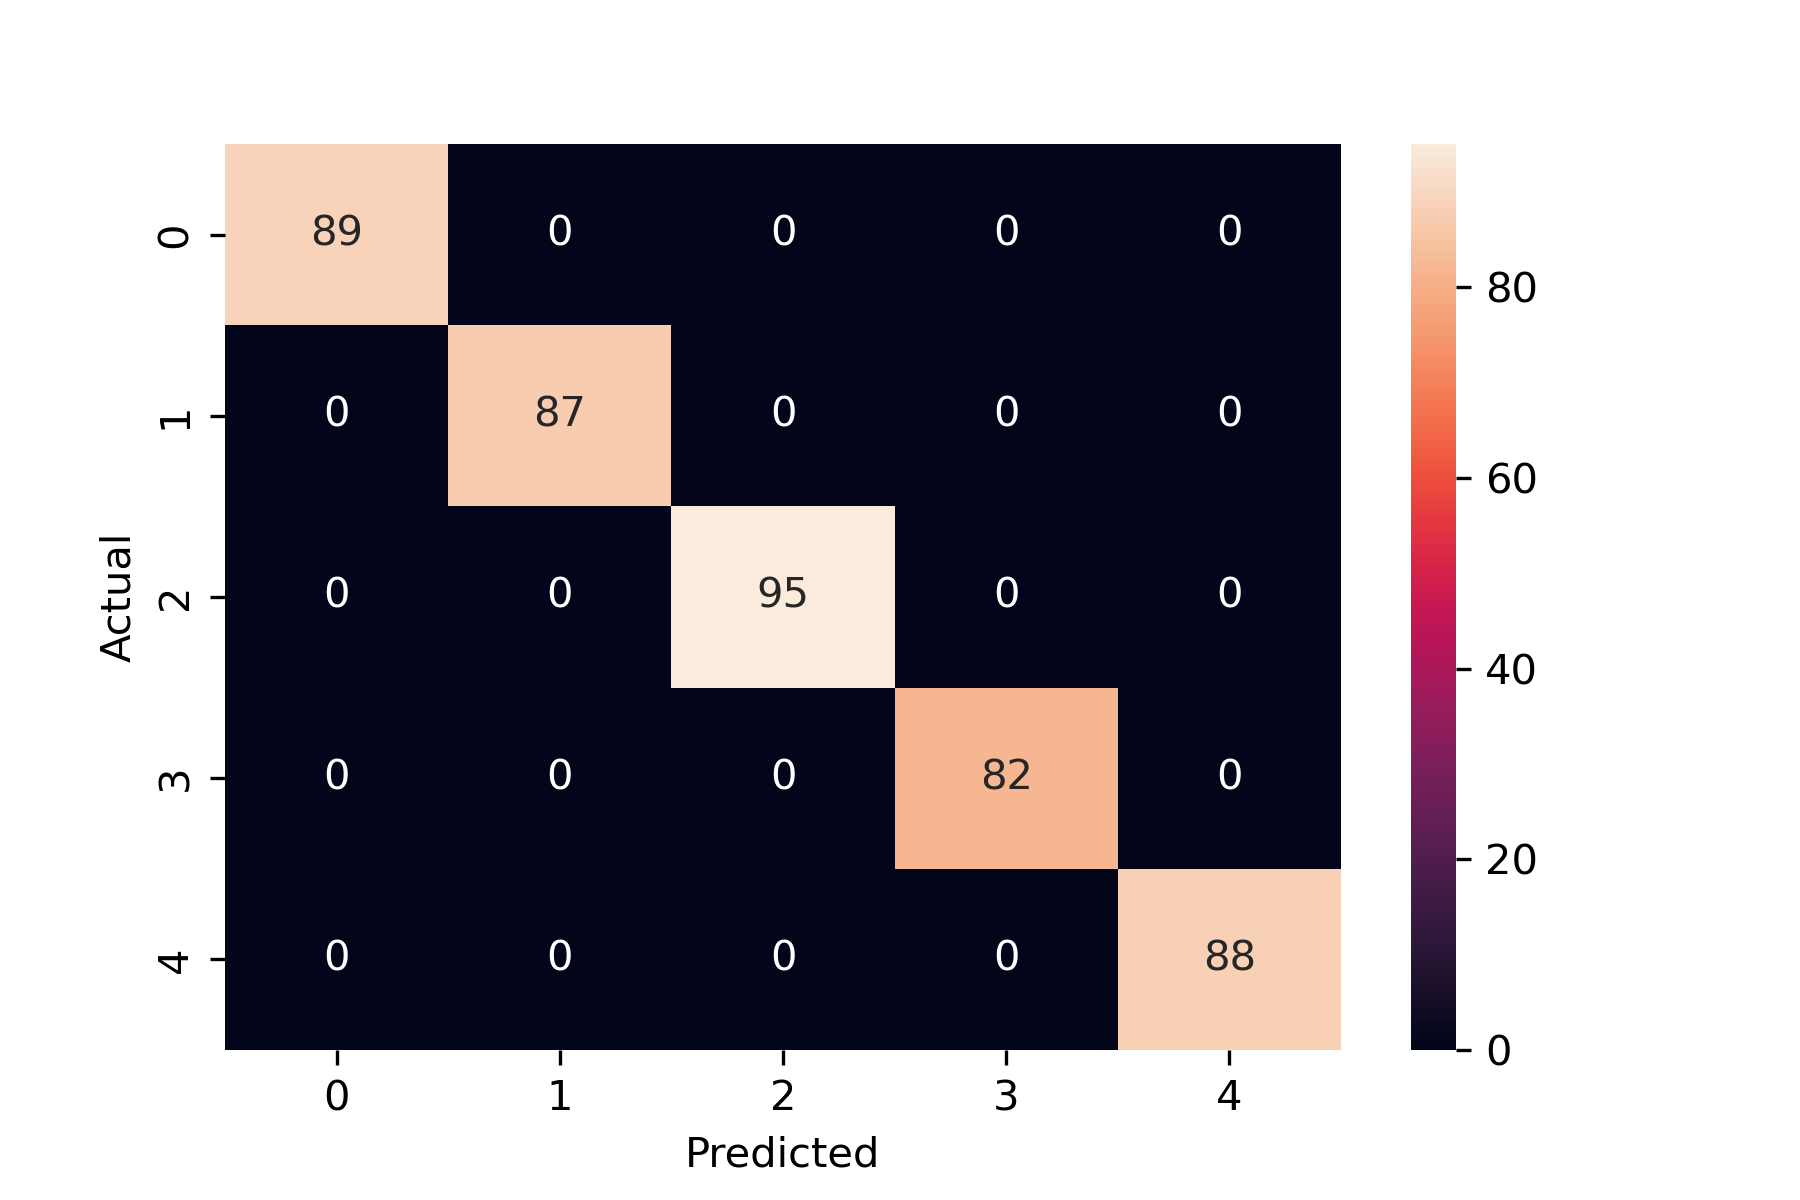
\includegraphics[width=.75\textwidth]{img/KNNplotNorm-SKLearn.png}
			\caption{Przykładowa macierz błędów}
			\label{fig:conf-matrix}
		\end{figure}
	
	\newpage
	\addcontentsline{toc}{section}{Część II}
    \section*{\relsize{1.5}Część II}
    
	\section{Opis działania}
	    \subsection{Wspólne}
        	Przed rozpoczęciem klasyfikacji zbiór danych należało podzielić na zbiór treningowy i testowy. Pierwszy z nich, traktowany jako znane dane, służy jako punkt odniesiena dla algorytmów, uczenia ich. Drugi zbiór traktowany był jako dane wprowadzane do programu w celu ich sklasyfikowania. Dzięki posiadaniu wiedzy o klasach, jakie przypisane były do tych próbek można było porównać je do wyników klasyfikacji i przeprowadzić analizę skuteczności algorytmów. Zwykle stosowane proporcje podziału to $7:3$, jednak testy przeprowadzane były także dla innych wartości.
        	
        	W przypadku, gdy dane w zbiorze są upporządkowane (tzn. poszczególne klasy występują w grupach), należy przed podziałęm zbioru przemieszać go w celu uzyskania wiarygodnych wyników. Pozwala to uniknąć sytuacji, w której w zbiorze testowym pojawią się klasy niewystępujące w zbiorze treningowym, których algorytm nie znał, a wieć nie miał możliwości poprawnie sklasyfikować.
        	
        	Kolejnym etapem była normalizacja wartości pojawiających się w zbiorze. Proces ten polega na przekształceniu wartości znajdujących się w pewnym przedziale na takie z przedziału $\langle 0;1 \rangle$, co w praktyce polega na wyszukaniu dla każdej cechy z osobna wartości największej i najmniejszej, a następnie przekształcenie każdej wartości zgodnie ze wzorem:
        	    $$x_{new}=\frac{x_{old}-min}{max-min}$$
        	
        	Po przeprowadzeniu klasyfikacji poszczególnymi algorytmami obliczone zostały miary wydajności pozwalające określić jakość algorytmów. W tym celu należy wprowadzić pojęcia (przy założeniu, że operujemy na dwóch klasach -- pozytywnej i negatywnej) wartości \textit{Prawdziwie Negatywnej} (\textit{TN} -- True Negative), czyli właściwie sklasyfikowanej jako negatywna, \textit{Prawdziwie Pozytywnej} (\textit{TP} -- True Positive), czyli właściwie sklasyfikowanej jako pozytywna oraz \textit{Fałszywie Negatywnej} (\textit{FN} -- False Negative) i \textit{Fałszywie Pozytywnej} (\textit{FP} -- False positive), czyli sklasyfikowane niepoprawnie, jako klasy przeciwne.
        	\begin{table}[h!]
        	    \centering
        	    \begin{tabular}{c c || c | c}
                    \multicolumn{2}{c}{} & \multicolumn{2}{c}{Sklasyfikowane} \\
                    ~ & ~ & Negatywne & Pozytywne \\
                    \hline \hline
                    \multirow{2}{5em}{Rzeczywiste} & Negatywne & TN & FP \\
                     & Pozytywne & FN & TP \\
                \end{tabular}
        	    \caption{Macierz błędów}
        	    \label{tab:matrix}
        	\end{table}
        	
        	Na podstawie tych wartości obliczone zostały miary:
        	\begin{itemize}
        	    \item \textbf{Dokładność (Accuracy)} -- jest to najbardziej intuicyjna miara określająca stosunek poprawnie sklasyfikowanych próbek do wszystkich próbek
        	        $$Accuracy=\frac{TP+TN}{TP+TN+FP+FN}$$
        	    
        	    \item \textbf{Precyzja (Precision)} -- stosunek prawidłowo skalsyfikowanych próbek pozytywnych do wszystkich próbek sklasyfikowanych jako pozytywne
        	        $$Precision=\frac{TP}{TP+FP}$$
        	   
        	    \item \textbf{Czułość (Recall)} -- stosunek próbek prawidłowo sklasyfikowanych jako pozytywne do wszystkich pozytywnych
        	        $$Accuracy=\frac{TP}{TP+FN}$$
        	    
        	    \item \textbf{F1} -- średnia ważona precyzji i czułości. W przypadku nierównomiernego rozkładu klas daje ona bardziej miarodajne wyniki przy założeniu, że wartości Fałszywe są na podobnym poziomie.
        	        $$F1=2*\frac{Precision * Recall}{Precision + Recall}$$
        	\end{itemize}
    	
        \subsection{algorytm KNN}
	        Algorytm k-najbliższych sąsiadów jest jednym z najprostszych algorytmów uczenia maszynowego. Opiera się na założeniu, że cechy rozpatrywanego przypadku są podobne do tych już znanych (ze zbioru treningowego). Na podstawie oceny odległości danej cechy od innych wartości, nadaje próbce taką samą klasę, jaką posiada największa liczba spośród zadanej ilości ($k$) sąsiadów.
	        
	        We własnej implementacji algorytmu, pierwszą wykonywaną czynnością jest określenie listy klas, jakie posiadają dane w zbiorze treningowym. Następnie obliacza jest odległość klasyfikowanej próbki od każdej pozycji w zbiorze treningowym. Do tego celu wykorzystano Odległość Minkowskiego. Przyjmuje się wtedy, że próbki są punktami w $n$-wymiarowej przestrzeni euklidesowej, gdzie n, to liczba branych pod uwagę cech:
	            $$X(x_1, x_2, \ldots, x_n), Y(y_1, y_2, \ldots, y_n) \in \mathbb{R}^n$$
	       Wtedy odległość między takimi punktami w przestrzeni oblicza się wg. wzoru:
	            $$D(X, Y)=\left(\sum_{i=1}^{n} |x_i-y_i|^m\right)^\frac{1}{m}$$
	       W zależności od parametru $m$ uzyskuje się różne odmiany Odległości Minkowskiego:
	       \begin{itemize}
	           \item dla $m=1$ będzie to odległość typu miejska/taksówkowa/Manhattan, liczona jako suma bezwzględnych różnich pomiędzy wspórzędnymi kartezjańskimi punktów.
	                $$D_1(X, Y)=\sum_{i=1}^{n} |x_i-y_i|$$
	           \item dla $m=2$ będzie to odległość euklidesowa, która jest odległością w lini prostej między punktami w przestrzeni euklidesowej.
	                $$D_2(X, Y)=\sqrt{\sum_{i=1}^{n} |x_i-y_i|^2}$$
	       \end{itemize}
	       
	       \begin{figure}[h!]
    			\centering
    			\label{minkowski-manhattan}
    			\subfloat[odległość Manhattan]{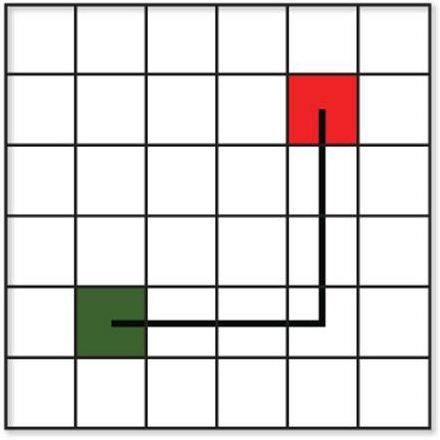
\includegraphics[width=.25\textwidth]{./img/metrics-1.jpg}}
    			\hfil
    			\label{minkowski-euklides}
    			\subfloat[odległość euklidesowa]{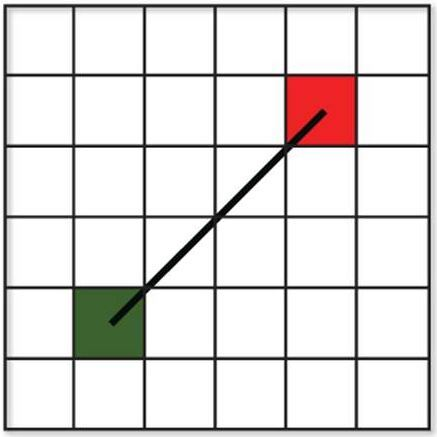
\includegraphics[width=.25\textwidth]{./img/metrics-2.jpg}}
    			\caption{Przedstawienie omawianych metryk w przestrzeni 2-wymiarowej}
    		\end{figure}
	       
	       Gdy zostaną wyznaczone wszystkie odległości, przeprowadzone zostaje głosowanie -- należy zliczyć ile spośród zadanych $k$ punktów, które leżą najbliżej próbki należy do każdej z klas, a następnie przypisać rozpatrywanej próbce klasę najliczniejszej grupy sąsiadów.
	       
	       Algorytm KNN jest algorytmem leniwego uczenia się -- nie generalizuje on danych, za każdym razem przeprowadza operacje na danych z zadanego zbioru treningowego. Algorytm ten wykorzystuje nadzorowaną technikę uczenia się, co oznacza, że dane treningowe są już sklasyfikowane i algoryt korzysta z tej klasyfikacji.
	    
	    \subsection{naiwny klasyfikator Bayesa}
	        Naiwny klasyfikator Bayesowski, bazujący na twierdzeniu Bayesa, nadaje się szczególnie do problemów o bardzo wielu wymiarach na wejściu. Mimo prostoty metody, często działa ona lepiej od innych, bardzo skomplikowanych metod klasyfikujących. Opisuje się go wzorem:
	            $$P(A|B)=\frac{P(B|A)P(A)}{P(B)}$$
	        gdzie:\\ $P(A|B)$ - Jak prawdopodobna jest hipoteza, mając skutek,\\$P(B|A)$ - Jak prawdopodobny jest dowód, zakładając że nasza hipoteza jest prawdziwa,\\ $P(A)$ - Jak prawdopodobna była nasza hipoteza przed zaobserwowaniem dowodów, \\ P(B) - Suma prawdopodobieństw wszystkich potencjalnych skutków zdarzenia:\\ $P(B)=\sum P(B|A)P(B)$ \\
	        
	        \begin{figure}[h!]
    			\center	
    			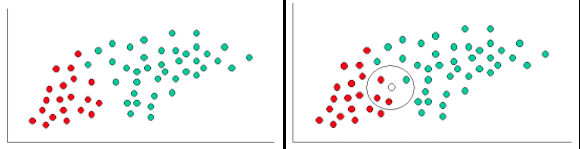
\includegraphics[width=.7\textwidth]{img/bayes_rysunek.png}
    			\caption{Sposób działania klasyfikatora Bayesa}
		    \end{figure} 
	        
	        Dla ilustracji koncepcji naiwnej metody Bayesa, rozpatrzmy przykład z powyższego rysunku. Jak widać, mamy tu obiekty zielone i czerwone. Naszym zadaniem będzie zaklasyfikowanie nowego obiektu, który może się tu pojawić.

            Ponieważ zielonych kółek jest dwa razy więcej niż czerwonych, rozsądnie będzie przyjąć, że nowy obiekt (którego jeszcze nie mamy) będzie miał dwa razy większe prawdopodobieństwo bycia zielonym niż czerwonym.
            
            W analizie Bayesowskiej, takie prawdopodobieństwa nazywane są prawdopodobieństwami a priori. Prawdopodobieństwa a priori wynikają z posiadanych, wcześniejszych (a priori) obserwacji. W tym wypadku, chodzi o procent zielonych względem czerwonych. Prawdopodobieństwa a priori często służą do przewidywania klasy nieznanych przypadków, zanim one się pojawią.
            
            Mając obliczone prawdopodobieństwa a priori, jesteśmy gotowi do zaklasyfikowania nowego obiektu (kółko białe). Ponieważ obiekty są dobrze pogrupowane sensownie będzie założyć, że im więcej jest zielonych (albo czerwonych) obiektów w pobliżu nowego obiektu, tym bardziej prawdopodobne jest, że obiekt ten ma kolor zielony (czerwony). Narysujmy więc okrąg wokół nowego obiektu, taki by obejmował, wstępnie zadaną liczbę obiektów (niezależnie od ich klasy). Teraz będziemy mogli policzyć, ile wewnątrz okręgu jest zielonych, a ile czerwonych kółek. Skąd obliczymy wielkość, którą można nazwać szansą.
            
            Jasne jest, że w powyższym przykładzie szansa, że X będzie czerwone jest większa niż szansa, że X będzie zielone.
            
            Mimo, że prawdopodobieństwo a priori wskazuje, że X raczej będzie zielone (bo zielonych jest dwa razy więcej niż czerwonych), to szanse są odwrotne, ze względu na bliskość czerwonych. Końcowa klasyfikacja w analizie Bayesowskiej bazuje na obu informacjach, wg reguły Bayesa.
            
            W rezultacie klasyfikujemy X jako czerwone, gdyż większe jest prawdopodobieństwo a posteriori takiej właśnie przynależności.\\
            
	        Różne naiwne klasyfikatory Bayesa różnią się głównie założeniami, jakie przyjmują w odniesieniu do rozkładu $P(x_{i}|y)$.
	        Uczący i klasyfikujący naiwni Bayes'i mogą być niezwykle szybcy w porównaniu z bardziej wyrafinowanymi metodami. Oddzielenie rozkładów cech warunkowych klas oznacza, że każdy rozkład może być niezależnie estymowany jako rozkład jednowymiarowy. To z kolei pomaga złagodzić problemy wynikające z przekleństwa wymiarowości.
            Z drugiej strony, chociaż naiwny Bayes jest znany jako przyzwoity klasyfikator, wiadomo, że jest złym estymatorem, więc wyników prawdopodobieństwa z przewidywanych próba nie należy traktować zbyt poważnie.
            
            W projekcie są używane trzy sposoby klasyfikacji dla naiwnego Bayesa:
            \begin{enumerate}
                \item Algorytm Gaussa - jest używany szczególnie wtedy, gdy cechy mają wartości ciągłe. Zakłada się również, że wszystkie cechy mają rozkład Gaussa, tj. rozkład normalny.
                $$ P(x_{i}|y)=\frac{exp(- \frac{(x_{i}- \mu_{y})^2}{2\sigma_{y}^2})}{\sqrt{2\pi \sigma_{y}^2}} $$
                gdzie $\mu$ to średnia arytmetyczna a $\sigma$ to odchylenie standardowe
                \item Algorytm Bernolliego - implementuje naiwne algorytmy uczenia i klasyfikacji Bayesa dla danych, które są dystrybuowane zgodnie z wielowymiarowymi rozkładami Bernoulliego tzn. może istnieć wiele cech, ale zakłada się, że każda z nich jest zmienną o wartości binarnej (Bernoulli, boolean). Dlatego ta klasa wymaga, aby próbki były reprezentowane jako wektory cech o wartościach binarnych; w przypadku przekazania innego rodzaju danych, instancja BernoulliNB może zbinaryzować swoje dane wejściowe (w zależności od parametru binaryzacji).\\ Zasada decyzyjna dla Bernoulliego naiwnego Bayesa opiera się na:
                $$ P(x_{i}|y) = P(i|y)x_{i}+(1-P(i|y))(1-x_{i}) $$
                \item Algorytm nienazwany - był on podany na kolokwium i wstępnie nie posiadał żadnej nazwy. Wzór jego to: 
                $$f(x)=\left\{
                \begin{array}{ccc}
                \frac{x-\mu}{6\sigma^2}+\frac{1}{\sqrt{6}\sigma}&\mbox{dla}&\mu-\sqrt{6}\sigma \leq x \leq \mu,\\
                \frac{-(x-\mu)}{6\sigma^2}+\frac{1}{\sqrt{6}\sigma}&\mbox{dla}&\mu < x \leq \mu+\sqrt{6}\sigma,\\
                0&\mbox{dla pozostałych}&\\
                \end{array}
                \right.$$
            \end{enumerate}
            
	    
	    \subsection{Perceptron}
            Perceptron jest prostym algorytmem uczenia maszynowego. Miał on odwzorowywać pracę pojedynczego neuronu. Perceptron otrzymuje próbkę danych wejściowych, która jest klasyfikowana, poprzez przypisanie  wag jej cechom. Aby to osiągnąć perceptron przechodzi przez fazy treningu i testowania. W fazie treningu wagi są inicjowane dowolną wartością. Następnie perceptron ocenia próbkę oraz porównuje swoją decyzję z rzeczywistą klasą próbki.


            Jeśli algorytm dokonał złej klasyfikacji, wagi są dostosowywane, aby lepiej pasowały do danej próbki. Proces jest powtarzany w kółko, by precyzyjnie zoptymalizować błędy systematyczne. Po tym algorytm jest gotowy do przetestowania z zestawem nieznanych mu próbek, by sprawdzić, czy wytrenowany model jest wystarczająco ogólny, aby poradzić sobie z innymi próbkami.


            Ten prosty opis od razu podsuwa potencjalne problemy:
            \begin{itemize}
                \item Model musi być przetrenowany przez dużą liczbę już sklasyfikowanych próbek. Czasem może wystarczyć ich kilkadziesiąt, a czasem potrzeba będzie nawet tysięcy próbek.
                \item Faza przetwarzania zająć się musi brakiem cech, nieskorelowanymi  danymi oraz skalowaniem.
                \item Perceptron potrzebuje próbek dających się oddzielić liniowo, w celu osiągnięcia zbieżności.
            \end{itemize}{}
            Reprezentując próbki jako wektory o rozmiarze n, gdzie n jest liczbą cech, perceptron może być modelowany przez złożenie dwóch funkcji. Pierwsza z nich, niech będzie to f(x), mapuje wektor cech wejściowych x na wartość skalarną przesuniętą o wartość b:
	    
	        $$
	        f(x)=\left\{
	        \begin{array}{ccc}
	        \mathbb{R}^{n} \rightarrow \mathbb{R}  \\
	        w  \cdot  x + b
	        \end{array} 
	        \right.$$
	        ,gdzie  $w  \cdot  x$ jest iloczynem skalarnym między w i x zdefiniowanym jako: $\sum_{i=1}^{n} w_i x_i $
	
	        Drugą funkcją predict(x), funkcja skokowa, zazwyczaj wykorzystuje się funkcje heavyside’a lub signum, mapuje wartość skalarną na wyjście binarne.
	        $$
	        predict(x) = sgn(f(x))=\left\{
        	\begin{array}{ccc}
	            1 & \mbox{jeśli} & f(x)\geq0\\
	            -1 & \mbox{dla pozostałych}\\
	        \end{array}
	        \right.$$
	
	
	\section{Algorytmy}
        \subsection{Wspólne}
            \subsubsection*{Normalizacja zbioru}
                \begin{algorithm}[H]
                    \KwData{$X$}
                    \KwResult{$XNorm$}
                    ~\\
                    // ustalenie wartości maksymalnej i minimalnej w kolumnie\\
                    \For{$i\gets0$ \KwTo $len(X[0])$}{
                        $max=max(X[:,i])$\\
                        $min=min(X[:,i])$\\
                        ~\\
                        // obliczenie nowej wartości w kolumnie dla wszystkich próbek\\
                        \For{$j\gets0$ \KwTo $len(X)$}{
                            $XNorm[j,i]=(X[j,i]-min)/(max-min)$\\
                        }
                    }
                    ~\\
                    \label{alg:normalize}
                    \caption{Algorytm normalizacji zbioru}
                \end{algorithm}
        
        \subsection{algorytm KNN}
            \subsubsection*{Odległość Minkowskiego}
                \begin{algorithm}[H]
                    \KwData{$v1$, $v2$, $m$}
                    \KwResult{D}
                    ~\\
                    $D = 0$\\
                    \For{$i\gets0$ \KwTo $len(v1)$}{
                        $D += abs(v1[i] - v2[i])**m$\\
                    }
                    $D = D**(1/m)$\\
                    ~\\
                    \label{alg:minkowski}
                    \caption{Algorytm Odległości Minkowskiego}
                \end{algorithm}
            
            \subsubsection*{Właściwy algorytm KNN}
                \begin{algorithm}[H]
                        \KwData{$sample$, $X$, $C$, $k$, $m$}
                        \KwResult{$result$}
                        ~\\
                        // utworzenie slownika na podstawie nazw klas\\
                        $classes = \{~\}$\\
                        \For{$i\gets0$ \KwTo $len(C)$}{
                            $classes[C[i]] = 0$\\
                        }
                        ~\\
                        \label{alg:KNN}
                    \end{algorithm}
                    \begin{algorithm}[H]
                        ~\\
                        // obliczenie odleglosci probki od kazdego rekordu w zbiorze\\
                        $distances = [~]$\\
                        \For{$i\gets0$ \KwTo $len(X)$}{
                            $distances~+=~D(sample, X[i], m)$\\
                        }
                        ~\\
                        // sortowanie (stogowe) zbioru wzgledem odleglosci\\
                        $heap = [~]$\\
                        \For{$i\gets0$ \KwTo $len(X)$}{
                            $heap~+=~(distances[i], X[i])$\\
                        }
                        ~\\
                        // glosowanie\\
                        \For{$i\gets0$ \KwTo $k$}{
                            $classes[heap.pop()] += 1$\\
                        }
                        $result = max(classes)$
                        ~\\
                        \caption{Algorytm KNN}
                    \end{algorithm}
        
        \subsection{naiwny klasyfikator Bayesa}
            \begin{algorithm}[H]
                    \KwData{$XTrain,XTest$}
                    \KwResult{$result$}
                    ~\\
                    $s=XTrain$\\
                    $\mu=XTest$\\
                    // pętla po każdym elemencie modelu treningowego\\
                    \For{$q\gets1$ \KwTo $s$}{
                    // inicjalizacja elementów modelu treningowego\\
                        $\mu[q]=0$} 
                        // pętla po każdym wektorze\\
                    \For{$j\gets1$ \KwTo $\mu$}{ 
                        // zwiększanie liczby wektorów dla wartości $x_{j.p}$ z wektora $x_{j}$\\
                        $\mu[d[j,p]]++$ \\
                        // pętla po każdym atrybucie\\
                        \For{$k\gets1$ \KwTo $p-1$}{ 
                            // zwiększanie liczby wektorów z wartościami $x_{j.k}$ oraz $x_{j.p}$\\
                            $z=\mu[\phi(k-1)+(d[j,k]-1)*\phi(0)+d[j,p]]$ \\
                            $z=z+1$
                        }
                    }
                    $result=z$
                    ~\\
                    \label{alg:bayes}
                    \caption{Algorytm Bayesa}
                \end{algorithm}
        
        \subsection{Perceptron}
            \begin{algorithm}[H]
		        \KwData{X, Y, N\_iter}
		        \KwResult{Brak //algorytm modyfikuje wartości w obiekcie}
		        //przyjęcie domyślnej wartości przesunięcia jako 0\\
		        $self.b=0$\;
		        //utworzenie tablicy wag równych zero\\
		        $self.w=np.zeros(x.shape[1]) $\;
		        //utworzenie pustej listy ilości źle sklasyfikowanych próbek\\
		        $self.misclassified\_samples=[~] $\;
		        //pętle dla wybranej ilości iteracji
		        \For{$i\gets0$ \KwTo $N\_iter $}{
			        //utworzenie licznika błędów dla bierzącej iteracji\\
			        errors=0\\
			        //pętla po każdej próbce\\
			        \For{$xi, yi$ \textbf{in}  $zip(X, Y) $}{
			            // obliczenie różnicy między przewidzianą wartością t(x),\\
			            //a prawdziwą wartością, przeskalowane przez learning rate(domyślnie$=0.1$)\\
			            $update = self.learning\_rate *(y_i - self.predict(x_i))  $\\
			            //aktualizacja wartości przesunięcia oraz tablicy wag\\
			            $self.b~+=~update $\\
			            $self.w~+=~update*x_i $\\
			            //jeśli przewidywana wartość jest poprawna, update będzie równy 0\\
			            $errors~+=~int(update != 0)$\\
			        }
			        //wpisanie do listy liczbę błędów w bierzącej iteracji\\
		            $self.missclasified\_samples.append(errors) $\\
		        }
		        \caption{Algorytm Perceptronu}
	        \end{algorithm}

	\section{Zbiór danych}
        Wykorzystany zbiór danych opiera się na informacjach zbieranych przez urządzenie \textit{Smart-Yoga Pillow} (\textit{SaYoPillow}). Ma ono na celu pomóc w zrozumieniu zależności pomiędzy parametrami snu, a poziomem stresu
	
	Zbiór danych posiada 630 unikatowych próbek oraz składa się z poszczególnych cech:
	\begin{itemize}
	    \item Pomiar chrapania - ilość wykonywania czynności chrapania podczas snu, im większe tym gorsze,
	    \item Pomiar oddechu - ilość wdychanego oraz wydychanego powietrza podczas snu, im większe tym gorsze,
	    \item Temperatura ciała - wysokość temperatury ciała podczas snu, im mniejsze tym gorsze,
	    \item Ruch kończyn - ilość samowolnych ruchów części ciała podczas snu, im większe tym gorsze,
	    \item Pomiar tlenu we krwi - ilość komórek tlenu we krwi, im mniejsze tym gorsze,
	    \item Ruch gałki ocznej - ilość samowolnego poruszania się gałek ocznych podczas snu, im większe tym gorsze,
	    \item Ilość snu - ilość godzin spędzonych podczas snu, im mniejsze tym gorsze,
	    \item Tętno pracy serca - szybkość pracy serca podczas snu, im większe tym gorsze,
	    \item Poziom stresu - ogólny wyznacznik poziomu stresu na podstawie powyższych zmiennych, wyznacza się poprzez wystawienia jednej liczby z zakresu od 0 do 4, gdzie 0 to najlepszy wynik -- minimalny poziom stresu, a 4 to najgorszy -- maksymalny poziom stresu.
	\end{itemize}
	
	
		    \begin{figure}[h!]
			\center	
			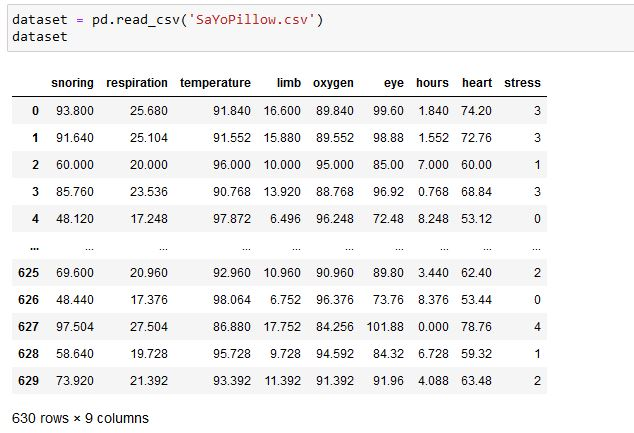
\includegraphics[width=.9\textwidth]{img/baza.JPG}
			\caption{Przykładowe dane w bazie}
		\end{figure}
		Jak widać powyżej dane są już potasowane, więc użycie metody tasowania nie jest tu potrzebne. Za to potrzebują one jak najbardziej normalizacji do lepszego i łatwiejszego odczytu.\\
		
		Natomiast wykresy poniżej to wynik użycia funkcji 'pairplot'. Wykreśla on relacje parami w zestawie danych.
        Domyślnie ta funkcja tworzy siatkę osi w taki sposób, że każda zmienna liczbowa w danych będzie współdzielona przez osie y w jednym wierszu i osie x w jednej kolumnie. Wykresy ukośne są traktowane inaczej: wykres rozkładu jednowymiarowego jest rysowany, aby pokazać marginalny rozkład danych w każdej kolumnie.
        
        Dzięki temu możemy zauważyć dużą kompatybilność danych między sobą oraz możemy wysnuć dobre wyniki względem dalszych etapów tego projektu.
		\begin{figure}[h!]
			\center	
			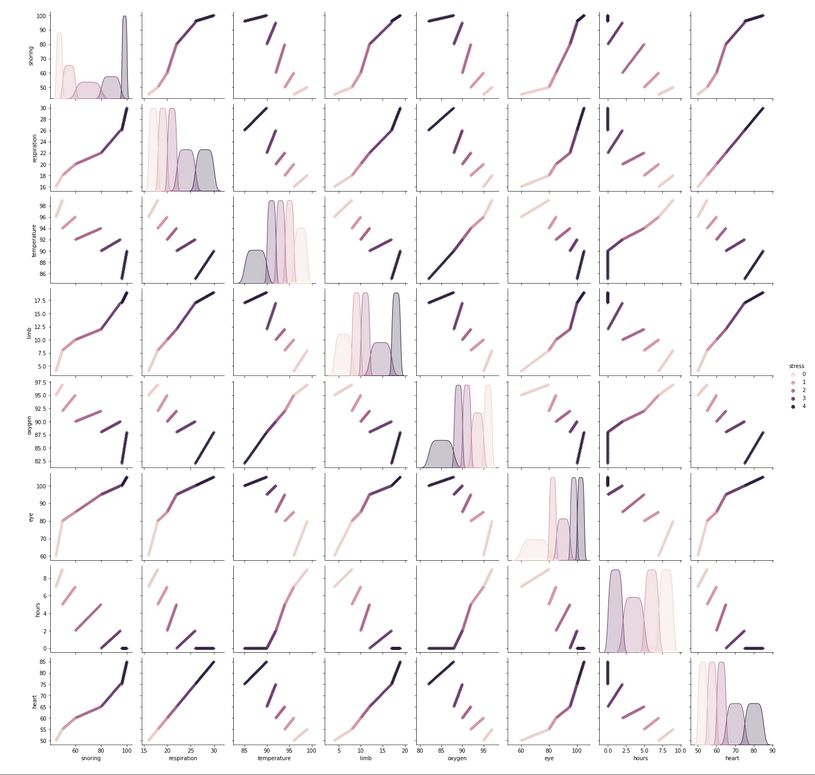
\includegraphics[width=1.1\textwidth]{img/pairplot.JPG}
			\caption{Pairplot}
		\end{figure}
	
	\pagebreak
	\section{Implementacja}
        \subsection{Wspólne}
            W implementacji algorytmów przygotowujących zbiór danych do klasyfikacji stworzono klasę \textit{DataProcessing} zawierającą wszystkie przydatne do tego metody:
            \begin{itemize}
                \item metoda \textit{shuffle()} przyjmująca jako argument zbiór danych. Zamienia ona pozycje w zbiorze miejscami przy użyciu generatora liczb pseudolosowych i zwraca przetasowany zbiór.
                
                \item metoda \textit{splitSet()} dzieląca zbiór na zbiory treningowy i testowy według ustalonej z góry proporcji
                
                \item metoda \textit{normalize()} normalizująca wartości w zbiorze zgodnie z algorytmem \ref{alg:normalize}.
                
                \begin{lstlisting}[language=Python, caption=metoda \textit{normalize()}, label=lst:normalize]
def normalize(x):
    x = x.copy()
    values = x.select_dtypes(exclude="object")
    columnNames = values.columns.tolist()
    columnNames.remove("stress")
    
    # znalezienie wartosci skrajnych w kolumnie
    for column in columnNames:
        data = x.loc[:,column]
        max1 = max(data)
        min1 = min(data)
        
        # normalizacja wartosci w kolumnie
        for row in range(len(x)):
            new Value=((x.at[row,column]-min1)/(max1-min1))
            x.at[row, column] = newValue
    return x
                \end{lstlisting}
            \end{itemize}
            
            Do importu oraz analizy zbioru użyto metod biblioteki \textit{pandas} oraz \textit{seaborn}. Wykorzystano także bibliotekę \textit{SKLearn} do wyznaczenia wskaźników wydajności oraz zaimplementowanych w niej klasyfikatorów w celu porównania ich z własnymi implementacjami.
        
        \subsection{algorytm KNN}
            W ramach implementacji stoworzono klasę \textit{KNN} zawerającą metody obliczające Odległość Minkowskiego oraz klasyfikujące.
            \begin{itemize}
                \item metoda \textit{metric()} -- oblicza Odległość Minkowskiego dla dwóch zadanych wektorów. W zależności od parametru $m$ otrzymywana jest odległość odpowiedniego typu.
                \begin{lstlisting}[language=Python, caption=metoda \textit{metric()}, label=lst:metric]
def metric(v1, v2, m):
    tmp = 0
    for i in range(len(v1)-1):
        tmp += abs(v1[i] - v2[i])**m
    return tmp**(1/m)
                \end{lstlisting}
                
                \item metoda \textit{classify()} -- klasyfikuje zadaną próbkę w oparciu o zbiór treningowy i podane klasy, liczbę sąsiadów i typ metryki zgodnie z algorytmem \ref{alg:KNN}
                \begin{lstlisting}[language=Python, caption=metoda \textit{classify()} w KNN, label=lst:classify]
def classify(sample, X, C, k, m):
    # utworzenie slownika na podstawie nazw klas
    classes = {}
    for cls in C:
        classes[cls] = 0
    
    # obliczenie odleglosci probki od kazdego rekordu w zbiorze
    distances = []
    for i in range(len(X)):
        distances.append(KNN.metric(sample, X.iloc[i], m))
    
    # sortowanie (stogowe) zbioru wzgledem odleglosci
    heap = []
    for i in range(len(X)):
        heappush(heap, (distances[i], X.iloc[i].stress))
    
    # glosowanie
    for i in range(0, k):
        classes[heappop(heap)[1]] += 1
    
    return max(classes, key = classes.get)
                \end{lstlisting}
                
            \end{itemize}
        
        \subsection{naiwny klasyfikator Bayesa}
            Do obliczeń w tym klasyfikatorze utworzono klasę \textit{NaiveBayes} posiadającą metody:
           \begin{itemize}
               \item \textit{mean()} przyjmująca pewne dane ze zbioru danych i obliczająca średnią arytmetyczną
               \item \textit{std()} przyjmująca pewne dane ze zbioru danych i obliczająca odchylenie standardowe
               \item \textit{fun()} przyjmująca argumenty ze zbioru danych oraz wcześniej obliczoną średnią jak także odchylenie standardowe i obliczająca klasyfikację z wybranego wzoru
               \item \textit{classify()} klasyfikująca wartości w zbiorze względem algorytmu \ref{alg:bayes}
               
                \begin{lstlisting}[language=Python, caption=metoda \textit{classify()} w Bayesie, label=lst:classify_B]
def classify(train,sample):
#separacja klas z bazy X
    names = train.stress.unique()
    classes = []
    for name in names:
        classes += [train[train['stress'] == name]]
        del classes[-1]['stress']
    #obl sred i odch dla kazdego atrybutu i klasy
    #obl skladowych prawdopodobienstw
    classes_fun = []
    for classy in classes:
        attrs_mean = []
        attrs_std = []
        attrs_fun = []
        for (name, data) in classy.iteritems():
            attrs_mean += [NaiveBayes.mean(data.values)]
            attrs_std += [NaiveBayes.std(data.values)]
            attrs_fun += [NaiveBayes.fun(sample[name],attrs_mean[-1],attrs_std[-1])]
        classes_fun += [np.prod(attrs_fun)]
    return names[classes_fun.index(max(classes_fun))]
                
                \end{lstlisting}
           \end{itemize}
            
        
        \subsection{Perceptron}
            Do implementacji Perceptronu utworzono klasę \textit{Perceptron} posiadającą metody:
	        \begin{itemize}
	            \item \textit{konstruktor} tworzy nowy perceptron, przyjmujący liczbę odpowiadającą za szybkość uczenia się, domyślnie przyjmuje 0.1
	            \item metoda \textit{f()} przyjmująca wektor cech, mapuje wektor na wartość skalarną
	            \item metoda \textit{predict()} przyjmuje wektor cech i wykorzystuje metodę \textit{f()}, konwertuje wartość skalarną na wyjście binarne
	            \item metoda \textit{fit()} dopasowuje model Perceptronu do treningowego zbioru danych
	   \begin{lstlisting}[language=Python,,caption=metoda \textit{fit()}, label=lst:fit]
def fit(self, x: np.array, y: np.array, n_iter=100):
    self._b = 0.0
    self._w = np.zeros(x.shape[1])
    self.misclassified_samples = []

    for _ in range(n_iter):
        # licznik bledow w aktualnej iteracji
        errors = 0
        for xi, yi in zip(x, y):
        # dla kazdej probki obliczana wartosc aktualizacji
            update = self.learning_rate * (yi - self.predict(xi))
            # dodanie jej do przesuniecia b oraz do tablicy wag
            self._b += update
            self._w += update * xi
            errors += int(update != 0.0)

        self.misclassified_samples.append(errors)
        \end{lstlisting}
	            \end{itemize}
        
	\section{Testy}
	
	    \subsection{algorytm KNN}
            Przeprowadzono testy dla dwóch metod obliczania odległości (dla $p=1$ oraz $p=2$) oraz kilku wartości $k$. Wykorzystano zarówno zbiór znormalizowany, jak i nieznormalizowany.
            
            Standardowo przyjmwaną liczbą sąsiadów $k$ jest $5$, jednak dla tej liczby algorytm okazał się mieć $100\%$ dokładność (Rysunek \ref{fig:conf-matrix-70}) niezależnie od pozostałych parametrów, dlatego przetestowano także większe wartości. Dopiero dla liczby sąsiadów $100$ klasyfikacja nieznormalizowanego zbioru przestaje dawać 100\% dokładność, jednak nadal są to róznice rzędu 1\%.
            
            \begin{figure}[h!]
    			\centering
    			\subfloat[$k=5$]{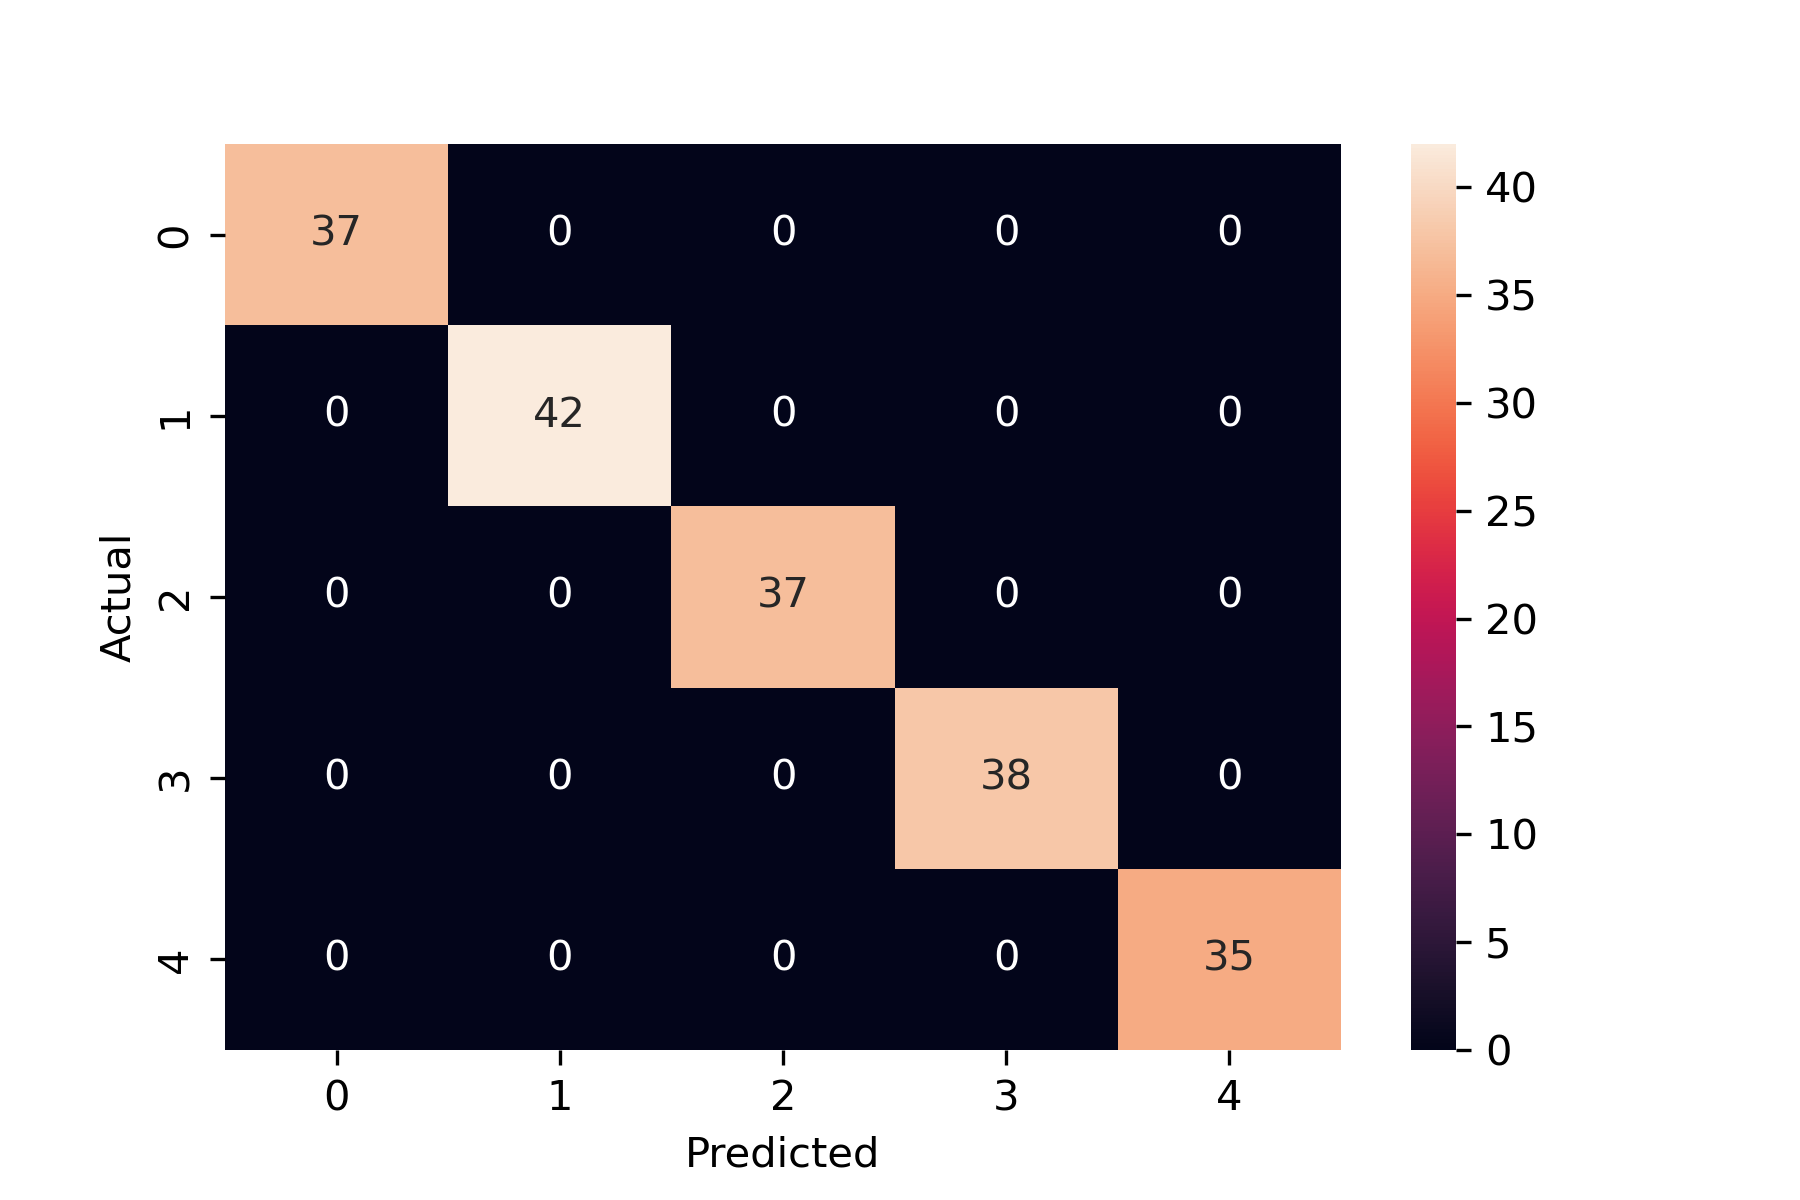
\includegraphics[width=.5\textwidth]{img/KNN/KNNplot-70-k5.png}}
    			\hfil
    			\subfloat[$k=100$, zbiór nieznormalizowany]{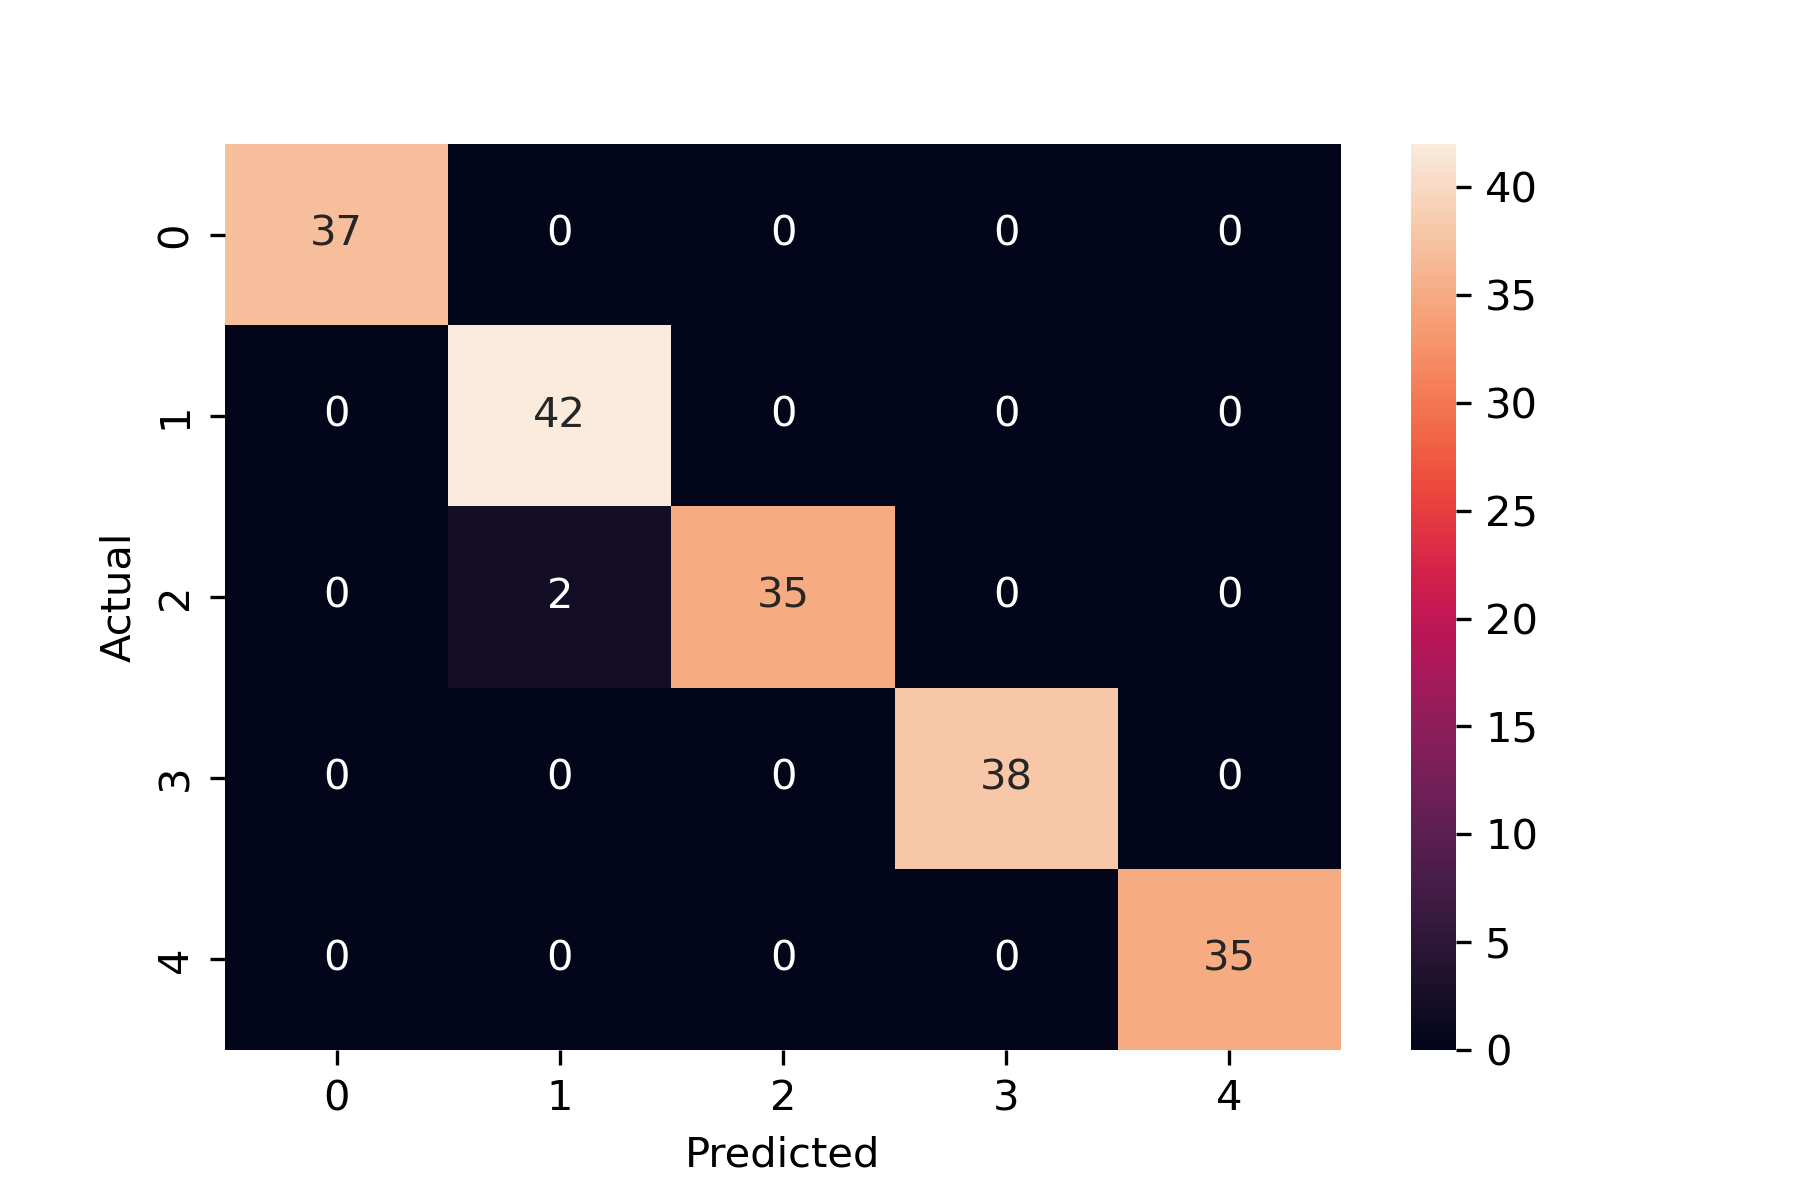
\includegraphics[width=.5\textwidth]{img/KNN/KNNplot-70-k100-nnorm.png}}
    			\caption{Macierze błędów dla podziału zbioru $70:30$}
    			\label{fig:conf-matrix-70}
    		\end{figure}
    		Metryki dla podziału $70:30$, $k=100$, zbioru nieznormalizowanego:
    		\begin{verbatim}
 Accuracy: 0.989
Precision: 0.990
   Recall: 0.989
       F1: 0.989
    		\end{verbatim}
    		
    		Ze względu na wysoką dokładność przeprowadzono także testy dla niestandardowego podziału zbioru -- $30:70$. W tym przypadku, ze względu na znacząco mniejszy zbiór treningowy jakość wyników spada znacznie szybciej, jednak nadal dla 5 sąsiadów klasyfikacja okazuje się bezbłędna.
    		\begin{figure}[h!]
    			\centering
    			\subfloat[$k=5$]{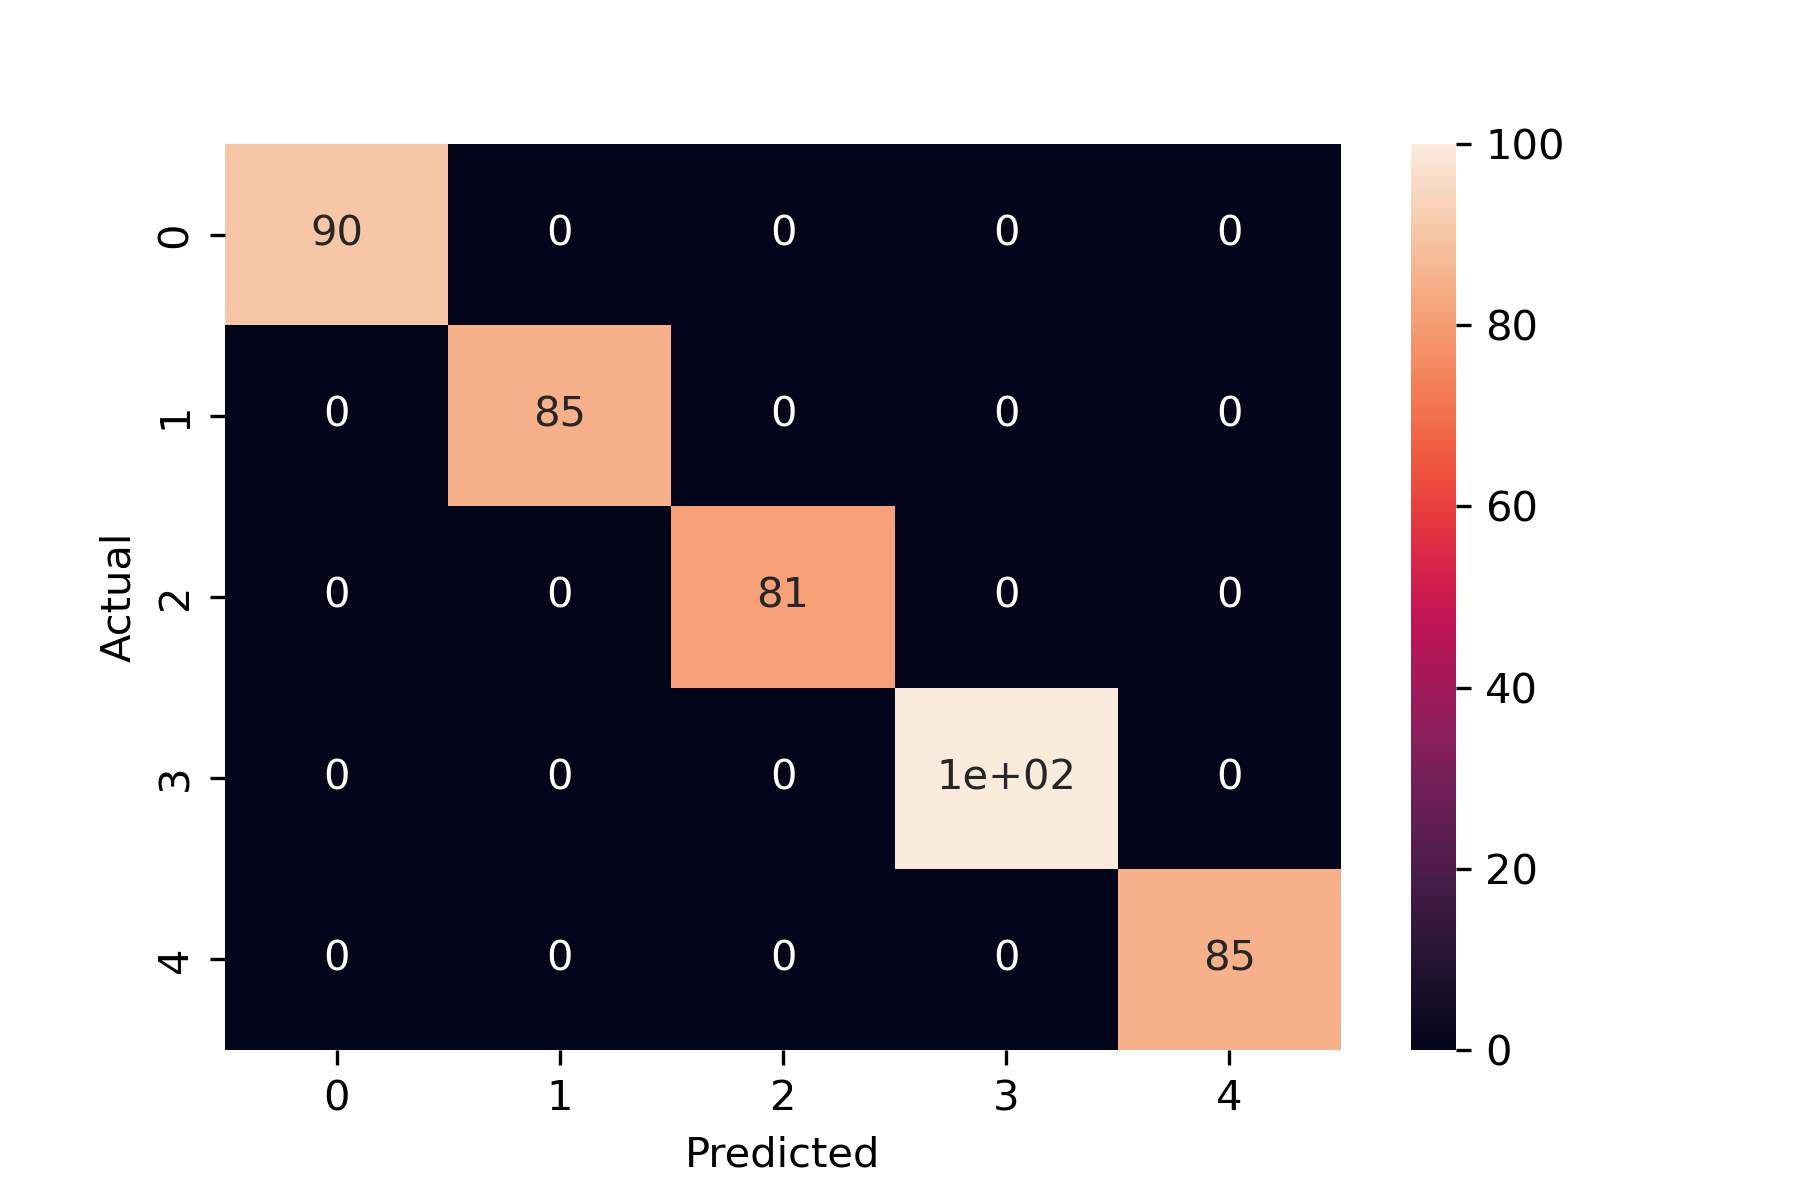
\includegraphics[width=.5\textwidth]{img/KNN/KNNplot30-k5.png}}
    			\hfil
    			\subfloat[$k=60$]{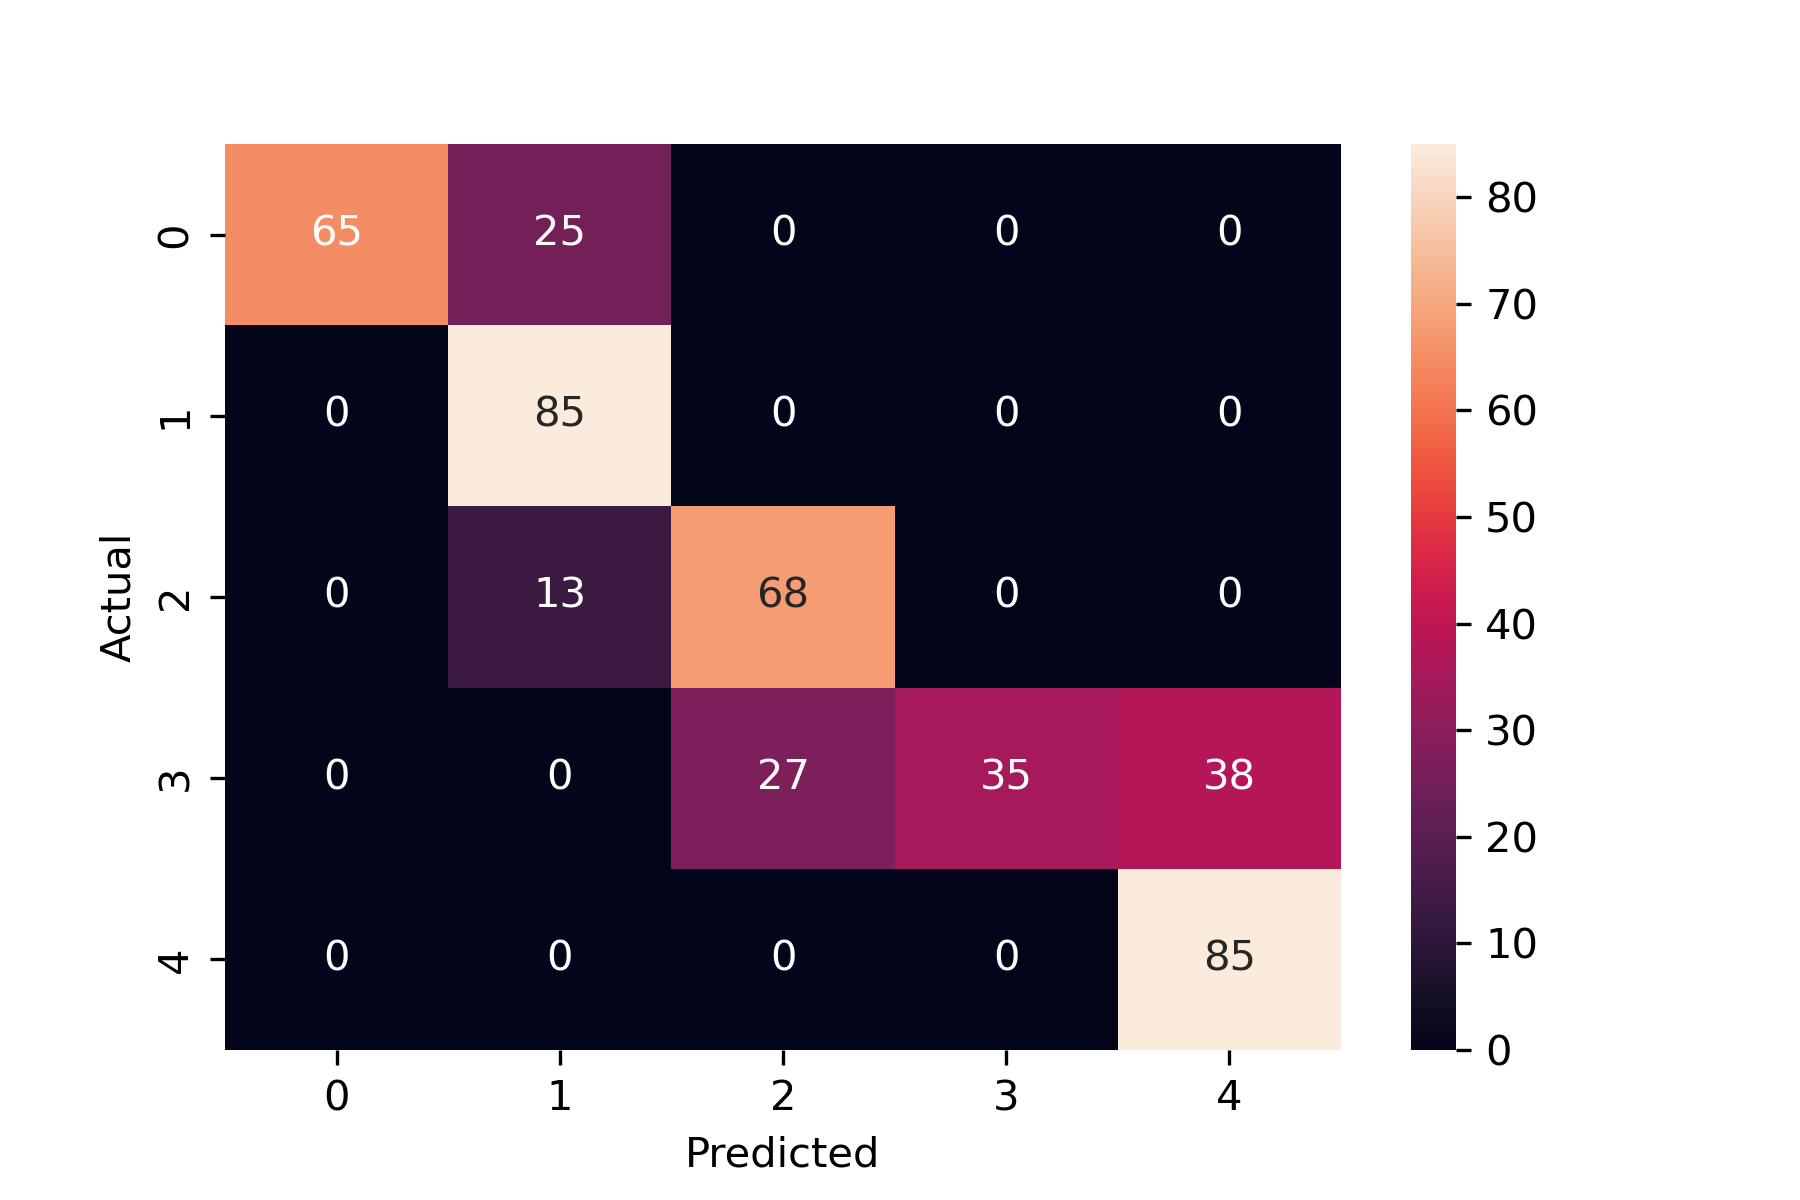
\includegraphics[width=.5\textwidth]{img/KNN/KNNplot-30-k60-nnorm.png}}
    			\caption{Macierze błędów dla podziału zbioru $30:70$}
    			\label{fig:conf-matrix-30}
    		\end{figure}
    		
    		W przypadku dużej liczby sąsidów wydajność spada, jednak otzymywane wyniki nie różnią się od siebie znacząco bez względu na użyty algorytm, metrykę, czy normalizację wzoru.
	    
	    \newpage
	    \subsection{naiwny klasyfikator Bayesa}
    	     \begin{figure}[h!]
        			\centering
        			\label{bayes_gauss_znorm}
        			\subfloat[Bayes przy użyciu Gaussa znormalizowanego]{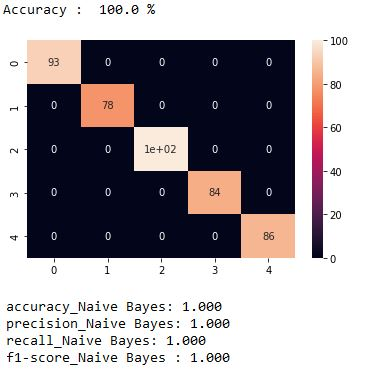
\includegraphics[width=.45\textwidth]{./img/bayes_gauss1.jpg}}
        			\hfil
        			\label{bayes_gauss_nieznorm}
        			\subfloat[Bayes przy użyciu Gaussa nieznormalizowanego]{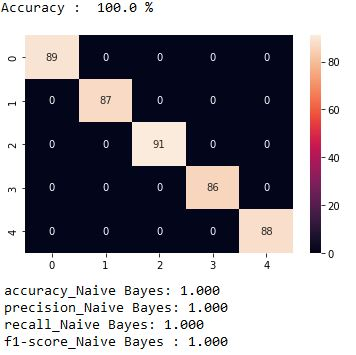
\includegraphics[width=.45\textwidth]{./img/bayes_gauss2.jpg}}
        			\caption{Bayes z algorytmem Gaussa}
     
        			\label{bayes_bernolli_znorm}
        			\subfloat[Bayes przy użyciu Bernolliego znormalizowanego]{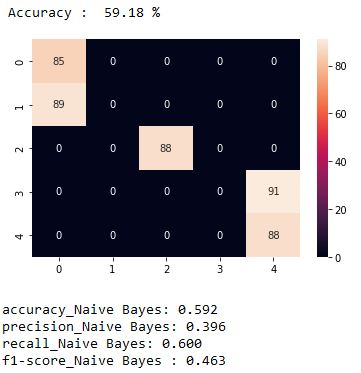
\includegraphics[width=.45\textwidth]{./img/bayes_bernolli1.jpg}}
        			\hfil
        			\label{bayes_bernolli_nieznorm}
        			\subfloat[Bayes przy użyciu Bernolliego nieznormalizowanego]{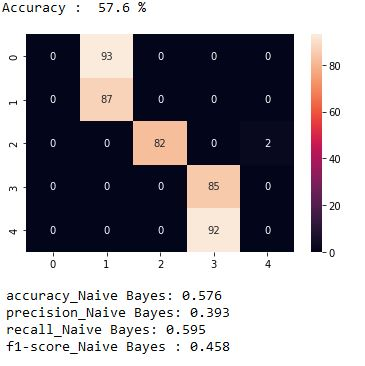
\includegraphics[width=.45\textwidth]{./img/bayes_bernolli2.jpg}}
        			\caption{Bayes z algorytmem Bernolliego}
        		\end{figure}
        		Jak możemy zauważyć przy użyciu algorytmu Gaussa wyniki otrzymujemy perfekcyjne z wynikiem 100\%. Jednak podczas użycia Bernolliego wyniki te spadają o niemalże połowę. Dowodzi to temu, iż lepszy oraz skuteczniejszy w przypadku tej bazy będzie wzór Gaussa w klasyfikatorze Bayesa.
    		
	    \subsection{Perceptron}
	        Przeprowadzono testy na próbce wybranej z przykładowego wykresu
	        \begin{figure}[h!]
	            \centering
	            \label{perceptron_podglad}
	            \subfloat[Podgląd rozkładu danych na podstawie trzech klas]{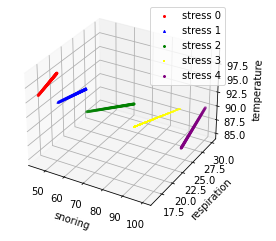
\includegraphics[width=.45\textwidth]{./img/perceptron/perceptron_ogolne.png}}
        		\hfil
        		\label{perceptron_zoom}
        		\subfloat[Ograniczenie wykresu do dwóch klas]{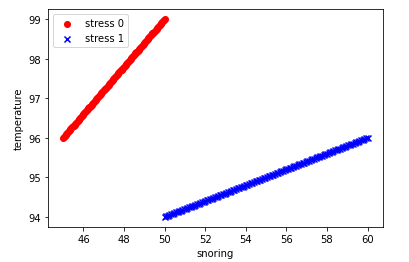
\includegraphics[width=.45\textwidth]{./img/perceptron/perceptron_zoom.png}}
        		\caption{Wybór próbki}
	        \end{figure}
	        \\
	        Trenowanie modelu:
	        \\
	        \begin{figure}[h!]
	            \centering
	            \label{perceptron_BS}
	            \subfloat[liczba wystąpień błędów przed standaryzacją]{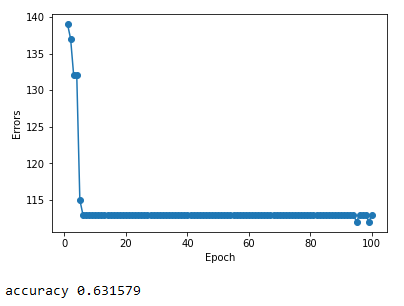
\includegraphics[width=.45\textwidth]{./img/perceptron/perceptron_errBS.png}}
        		\hfil
        		\label{perceptron_AS}
        		\subfloat[liczba wystąpień błędów po standaryzacji]{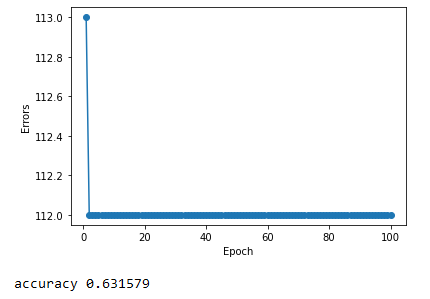
\includegraphics[width=.45\textwidth]{./img/perceptron/perceptron_errAS.png}}
        		\caption{Ilość błędów w trenowanym modelu}
	        \end{figure}
	        \\
	        Pomimo standaryzacji, wykresy różnią się od siebie w głównej mierze zakresem występowanych wartości.
	        W obu przypadkach dokładność modelu jest taka sama. Prawdopodobnie jest to spowodowane zbyt małą próbką danych.
	        \\
	        \begin{figure}
	            \centering
	            \subfloat[klasy przed standaryzacją]{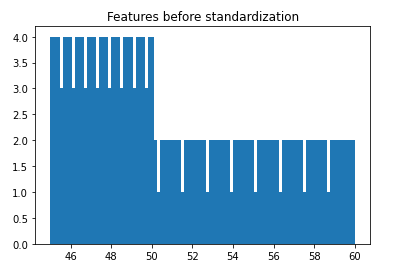
\includegraphics[width=.45\textwidth]{./img/perceptron/perceptron_BSAS-before.png}}
	            \subfloat[klasy po standaryzacji]{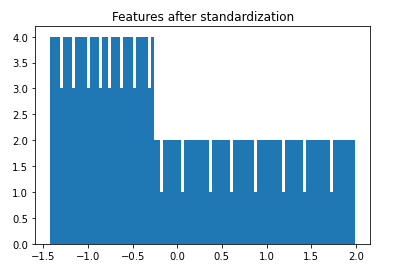
\includegraphics[width=.45\textwidth]{./img/perceptron/perceptron_BSAS-after.png}}
        		\caption{Skalowanie modelu}
        		\label{perceptron_FeatureScaling}
	        \end{figure}
	        \begin{figure}[h!]
        			\centering
        			\label{perceptron_wykres1}
        			\subfloat[Perceptron przy splicie 85:15]{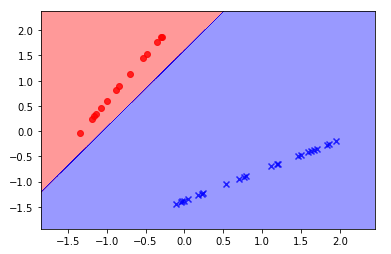
\includegraphics[width=.45\textwidth]{./img/perceptron/perceptron_Split15.png}}
        			\hfil
        			\label{perceptron_wykres2}
        			\subfloat[Perceptron przy splicie 80:20]{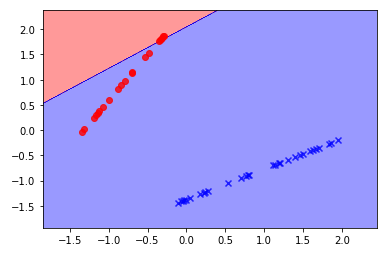
\includegraphics[width=.45\textwidth]{./img/perceptron/perceptron_Split20.png}}
     
        			\label{perceptron_wykres3}
        			\subfloat[Perceptron przy splicie 75:25]{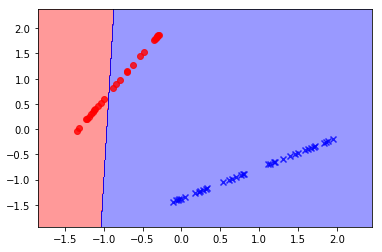
\includegraphics[width=.45\textwidth]{./img/perceptron/perceptron_Split25.png}}
        			\hfil
        			\label{perceptron_wykres4}
        			\subfloat[Perceptron przy splicie 70:30]{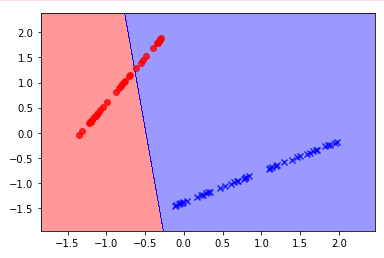
\includegraphics[width=.45\textwidth]{./img/perceptron/perceptron_Split30.png}}
        			\caption{Wizualizacja przewidywań modelu}
        		\end{figure}
	            Na podstawie poniższych obrazów widać, że najoptymalniejszym podziałem danych wejściowych jest 85:15. 
	            Przetestowano wpływ zwiększenia ilości iteracji oraz wpływu różnych prędkości uczenia. W obu przypadkach wpływ był niezauważalny na rezultat końcowy, co podtrzymuje teorię o zbyt małej próbce danych, jako że jest to jedyny element którego nie dało się zwiększyć.
	        
	\section{Eksperymenty}
	
        \subsection{algorytm KNN}
        
            W Tabeli \ref{tab:KNN} przedstawiono wskaźniki wydajności uzyskane przy podziale zbioru w niestandardowej proporcji $30:70$ oraz przy użyciu metryki euklidesowej.
            \begin{table}[h!]
        	    \centering
        	    \begin{tabular}{r || c | c | c | c}
        	        & nNorm & norm & SKL nNorm & SKL norm\\
        	        \hline
                    ~ & \multicolumn{4}{c}{$k=5$}\\
                    \hline
                    Accuracy & 1.00 & 1.00 & 1.00 & 1.00\\
                    Precision & 1.00 & 1.00 & 1.00 & 1.00\\
                    Recall & 1.00 & 1.00 & 1.00 & 1.00\\
                    F1 & 1.00 & 1.00 & 1.00 & 1.00\\
                    \hline \hline
                    ~ & \multicolumn{4}{c}{$k=20$}\\
                    \hline
                    Accuracy & 0.984 & 1.000 & 0.982 & 1.000\\
                    Precision & 0.985 & 1.000 & 0.983 & 1.000\\
                    Recall &  0.984 & 1.000 & 0.982 & 1.000\\
                    F1 &  0.984 & 1.000 & 0.982 & 1.000\\
                    \hline \hline
                    ~ & \multicolumn{4}{c}{$k=40$}\\
                    \hline
                    Accuracy & 0.930 & 1.000 & 0.930 & 0.995\\
                    Precision & 0.937 & 1.000 & 0.937 & 0.995\\
                    Recall & 0.930 & 1.000 & 0.930 & 0.995\\
                    F1 & 0.929 & 1.000 & 0.929 & 0.995\\
                    \hline \hline
                    ~ & \multicolumn{4}{c}{$k=60$}\\
                    \hline
                    Accuracy & 0.766 & 0.787 & 0.782 & 0.814\\
                    Precision & 0.829 & 0.855 & 0.837 & 0.879\\
                    Recall & 0.766 & 0.787 & 0.782 & 0.814\\
                    F1 & 0.746 & 0.742 & 0.760 & 0.769\\
                \end{tabular}
        	    \caption{wskaźniki wydajności algorytmu KNN}
        	    \label{tab:KNN}
        	\end{table}
        	
        	Wdajność algorytmów przy danej liczbie sąsiadów nie różni się znacząco. Różnice na poziomie $0.2\%$ można uznać za pomijanie małe.
        	
        	Przy porównaniu klasyfikacji zbbioru nieznormalizowanego ze znormalizowanym, algorytm zawsze lepiej radził sobie z danymi znormalizowanymi, różnice na podobnym poziomie ok. $2\%$.
        	
        	Otrzymane wyniki świadczą o bardzo dużej przydatności algorytmu KNN do klasyfikacji próbek w użytym zbiorze. Na ich otrzymanie z pewnością wpływ ma rozkład danych, które ostro przechodzą z jednej kalsy w drugą, co ułatwia prawidłową klasyfikację.
        	
        	Zauważalną różnicą własnej implementacji od gotowego rozwiązania jest czas trwania obliczeń przy własnym algorytmie wynoszący nawet kilkanaście sekund, podczas gdy algorytm biblioteki \textit{SKLearn} kończy pracę po ok. sekundzie.
	
	    \newpage
        \subsection{naiwny klasyfikator Bayesa}
       
        	\begin{figure}[h!]
        			\center	
        			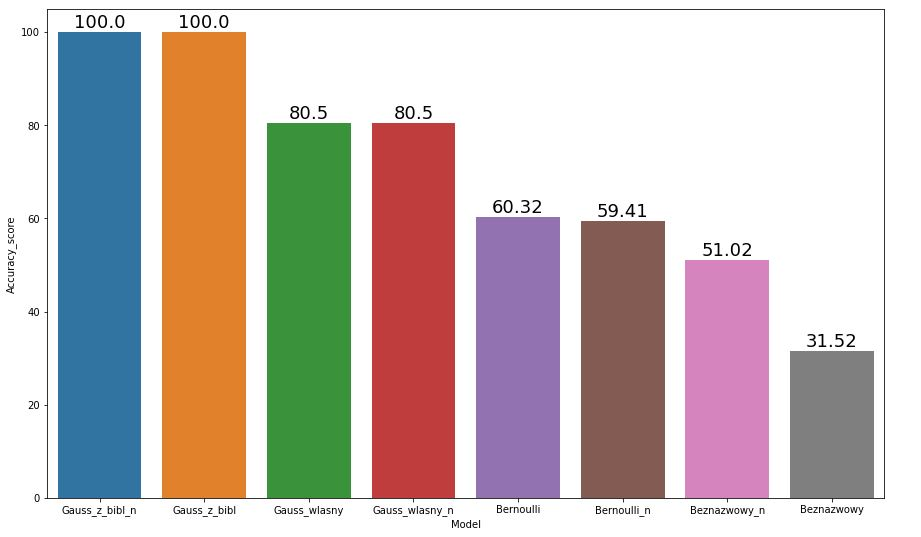
\includegraphics[width=1.1\textwidth]{img/bayes_zbiorczy.JPG}
        			\caption{Wyniki zbiorcze wielu metod Bayesa}
        		\end{figure}
        		Do wykonania powyższego wykresu zostały użyte 4 różne wzory do obliczenia klasyfikacji Bayesa: Gauss własnoręcznie zaimplementowany, Gauss zapożyczony z zewnętrznej biblioteki, Bernolli również zapożyczony z zewnętrznej biblioteki oraz ostatni bez nadanej mu nazwy (w tym przypadku nazwałem go "Beznazwowy"). Każdy wzór był poddany danymi znormalizowanymi oraz nieznormalizowanymi (znormalizowane mają dopisek '\_n' w nazwie.
        		
        		Owe wyniki jasno sugerują, które metody działają najlepiej w tej konkretnej bazie danych. Oczywiście nie można brać pod poważną uwagę pierwszych dwóch wyników, gdyż są one zbyt "idealne". Jak wiadomo jest bardzo mała szansa, że dostaniem maksymalną precyzję pomiarów danych, lecz to nie uświadamia o fałszywości owych wyników.
        		
        		Dalsze oceny precyzji są już na zadowalającym poziomie dla prawidłowej analizy. Można zauważyć, że poza jednym przypadkiem znormalizowane oraz nieznormalizowane dane praktycznie się od siebie nie różnią. Może to wynikać z dobrej jakości danych w samej bazie.
        
	
	\newpage
	\addcontentsline{toc}{section}{Część III}
    \section*{\relsize{1.5}Część III}
    
    \section{Pełny kod programu}
        \subsection{Algorytm KNN}
            \lstinputlisting[language=Python, caption=Kod algorytmu KNN]{./kod/Projekt_SSI-KNN.py}
        
        \subsection{Naiwny klasyfkator Bayesa}
            \lstinputlisting[language=Python, caption=Kod klasyfikatora Bayesa]{./kod/Projekt_SSI-Bayes.py}
        
        \subsection{Perceptron}
            \lstinputlisting[language=Python, caption=Kod perceptronu]{./kod/Projekt-SSI-Perceptron.py}
    
    
    \pagebreak
    \addcontentsline{toc}{section}{Literatura}
    
    \begin{thebibliography}{9}
        \bibitem{pillow-1}
            L. Rachakonda, A. K. Bapatla, S. P. Mohanty, and E. Kougianos,
            \emph{SaYoPillow: Blockchain-Integrated Privacy-Assured IoMT Framework for Stress Management Considering Sleeping Habits}.
            IEEE Transactions on Consumer Electronics (TCE), Vol. 67, No. 1, Feb 2021, pp. 20-29.
        
        \bibitem{pillow-2}
            L. Rachakonda, S. P. Mohanty, E. Kougianos, K. Karunakaran, and M. Ganapathiraju,
            \emph{Smart-Pillow: An IoT based Device for Stress Detection Considering Sleeping Habits}.
            in Proceedings of the 4th IEEE International Symposium on Smart Electronic Systems (iSES), 2018, pp. 161--166. 
    
    \end{thebibliography}
\end{document}
